\section{Results}
This section reports the descriptive and exploratory results produced by the
validated V9 metric artifacts. Results are organized by research question and
retain the analytical grain of each metric; no claim combines incompatible
grains or treats self-reported evidence as behavioral telemetry.

\subsection{RQ1: How do student developers utilize Generative AI, and how does this adoption shape their longitudinal perceptions of software engineering roles and project expectations?}

RQ1 is supported by two distinct evidence streams: the M1 survey panel,
which summarizes six perception families and separately reports self-reported
AI use, and M2, which summarizes perceived disruption agreement for six
software-engineering roles. All six cohort-by-semester/checkpoint cells in M1
have complete item coverage, with 46, 41, and 40 respondents in 2025.2 and
22, 20, and 18 respondents in 2026.1 at $T_1$, $T_2$, and $T_3$, respectively.
These are repeated cohort summaries, not an identified individual longitudinal
panel.
% PROVENANCE: M1 values and coverage are from
% paper_v9/data/metrics/m1_rq1_perception_panel_long.csv and
% paper_v9/data/metrics/m1_rq1_perception_panel.metadata.json. The executed
% verification notebook is paper_v9/verification_notebooks/verify_m1.ipynb.

The six perception families do not move as a single trajectory. These item
means use the inherited $0$--$4$ score scale, except for the separately
reported autonomy/tool-balance item, which uses its observed $1$--$5$ response
scale. Values below are reported as mean $\pm SD$. In 2025.2, mean AI benefit
increases from $2.13 \pm 1.00$ at $T_1$ to $2.25 \pm 0.90$ at $T_3$, while
five-year career impact decreases from $1.48 \pm 1.01$ to $1.33 \pm 0.83$.
Autonomy/tool balance changes from $3.09 \pm 0.89$ to $3.23 \pm 0.95$. In
2026.1, AI benefit decreases from $2.00 \pm 1.07$ to $1.56 \pm 0.98$,
whereas autonomy/tool balance increases from $2.64 \pm 0.85$ to
$3.44 \pm 0.92$, and five-year career impact changes from $1.55 \pm 0.91$
to $1.67 \pm 0.91$. The project-expectation families remain comparatively
low: at $T_3$, project challenges average $0.15 \pm 0.36$ in 2025.2 and
$0.06 \pm 0.24$ in 2026.1, while project feeling averages $0.35 \pm 0.77$
and $0.50 \pm 0.86$, respectively. These values describe
distinct response families and should not be interpreted as one latent measure
of AI dependence.

Figure~\ref{fig:rq1-m1} presents these six families with cohort-specific
standard-deviation bars. Table~\ref{tab:rq1-m1-endpoints} reports the
corresponding endpoint values in compact form.

\begin{figure*}[t]
\centering
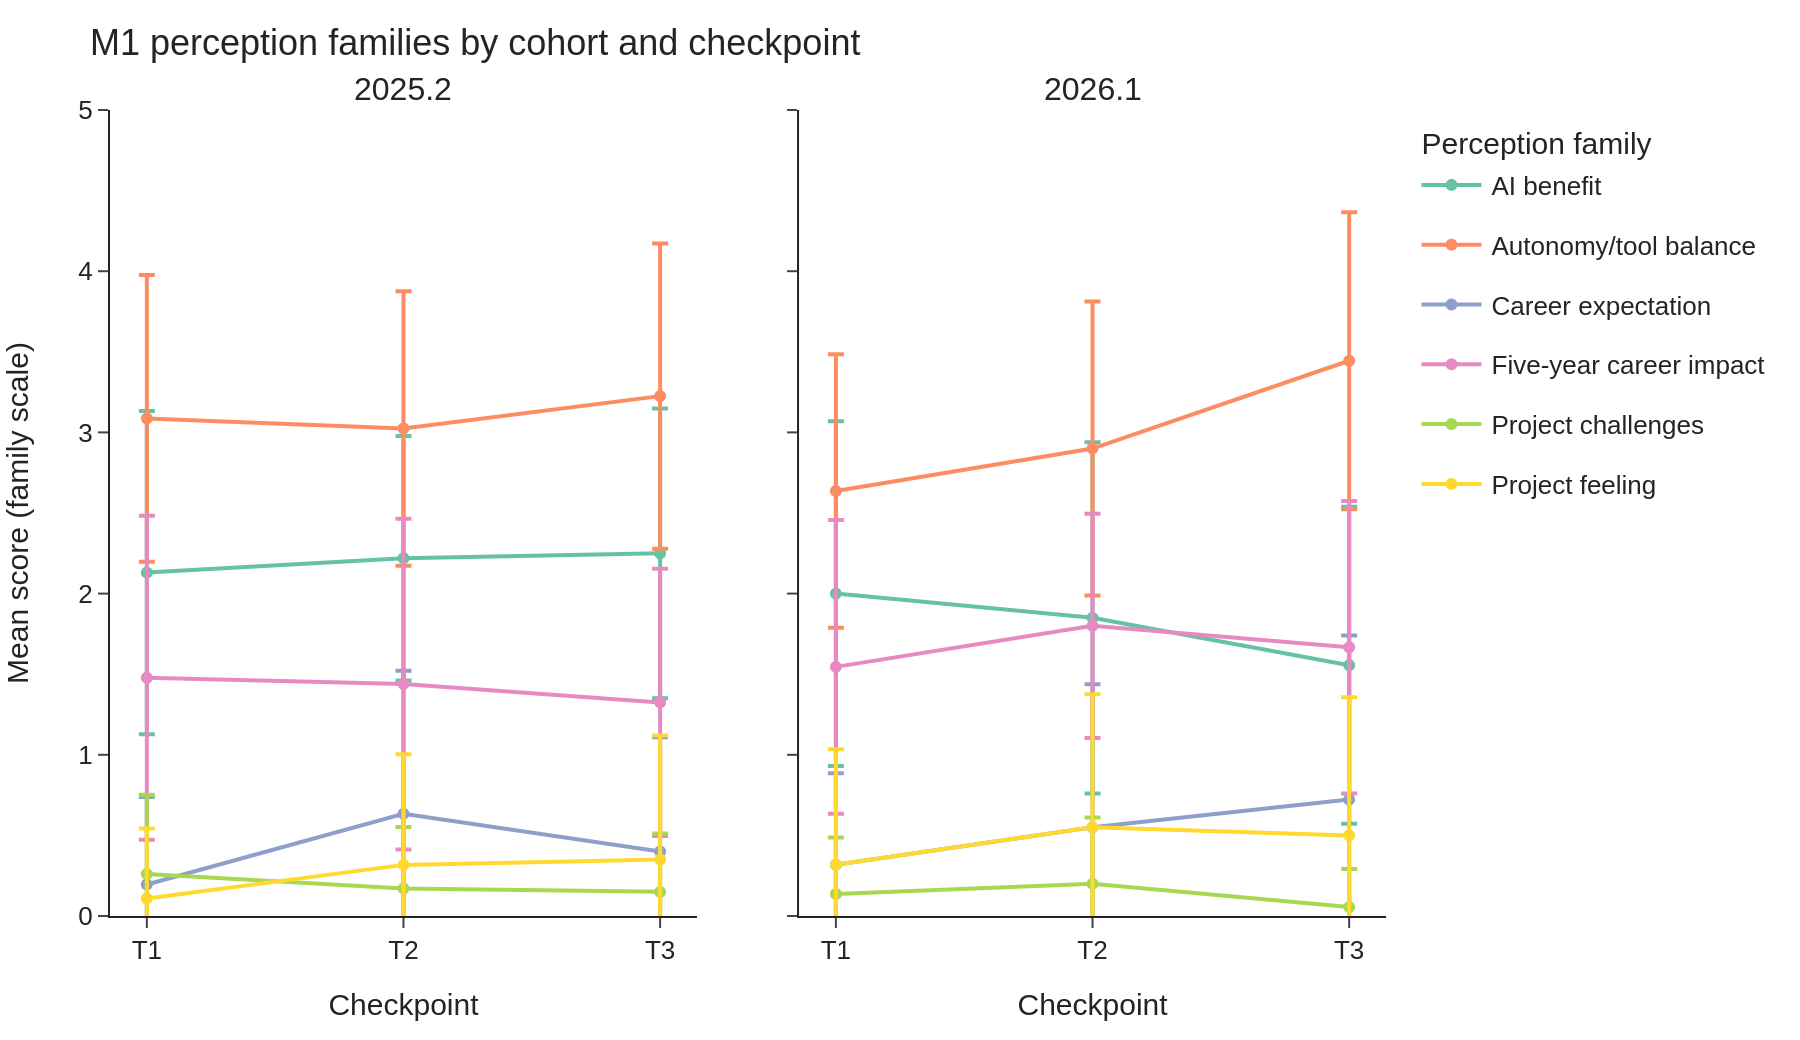
\includegraphics[width=\textwidth]{../figures/rq1_m1_perception_with_sd.png}
\caption{M1 perception families by cohort and checkpoint. Points show means
and bars show one standard deviation; family scales are retained from the
underlying instruments.}
\label{fig:rq1-m1}
\end{figure*}

\begin{table*}[t]
\caption{M1 Endpoint Summaries: Mean $\pm SD$}
\label{tab:rq1-m1-endpoints}
\centering
\scriptsize
\setlength{\tabcolsep}{4pt}
\begin{tabular}{@{}lcccc@{}}
\toprule
\textbf{Family} & \textbf{2025.2 $T_1$} & \textbf{2025.2 $T_3$} & \textbf{2026.1 $T_1$} & \textbf{2026.1 $T_3$} \\
\midrule
AI benefit & 2.13 $\pm$ 1.00 & 2.25 $\pm$ 0.90 & 2.00 $\pm$ 1.07 & 1.56 $\pm$ 0.98 \\
Five-year career impact & 1.48 $\pm$ 1.01 & 1.33 $\pm$ 0.83 & 1.55 $\pm$ 0.91 & 1.67 $\pm$ 0.91 \\
Autonomy/tool balance & 3.09 $\pm$ 0.89 & 3.23 $\pm$ 0.95 & 2.64 $\pm$ 0.85 & 3.44 $\pm$ 0.92 \\
Project challenges & 0.26 $\pm$ 0.49 & 0.15 $\pm$ 0.36 & 0.14 $\pm$ 0.35 & 0.06 $\pm$ 0.24 \\
Project feeling & 0.11 $\pm$ 0.43 & 0.35 $\pm$ 0.77 & 0.32 $\pm$ 0.72 & 0.50 $\pm$ 0.86 \\
\bottomrule
\end{tabular}
\end{table*}
% PROVENANCE: Table~\ref{tab:rq1-m1-endpoints} is transcribed from
% paper_v9/data/metrics/m1_rq1_perception_panel_long.csv. Figure~\ref{fig:rq1-m1}
% and its derived data are generated by
% paper_v9/scripts/results/generate_rq1_visuals.py.

The raw usage fields provide a separate adoption description. The share
reporting daily general AI use rises from $41.3\%$ to $45.0\%$ in 2025.2 and
from $54.5\%$ to $61.1\%$ in 2026.1 between $T_1$ and $T_3$. For software
projects specifically, the daily-use share changes from $23.9\%$ to $32.5\%$
in 2025.2 and from $40.9\%$ to $38.9\%$ in 2026.1. The most frequently
reported tasks include general research/questions, code generation, debugging,
and documentation. For example, code generation rises from $65.2\%$ to
$77.5\%$ in 2025.2, while documentation is reported by $72.7\%$ of the
2026.1 $T_1$ respondents and by $66.7\%$ at $T_3$. These are self-reported
frequencies and selected activities, not instrumented measures of tool use.
% PROVENANCE: usage frequency, task, tool, prior-experience, and autonomy
% values are persisted in paper_v9/data/metrics/m1_rq1_usage_frequency.csv,
% m1_rq1_usage_tasks.csv, m1_rq1_usage_tools.csv,
% m1_rq1_prior_ai_project_experience.csv, and
% m1_rq1_autonomy_tool_balance.csv.

Reported tool use is concentrated in a small group of widely named tools but
is not constant across cohorts. ChatGPT is reported by all 2025.2 respondents
at $T_1$ and $T_3$, and by $83.3\%$ of the 2026.1 $T_3$ respondents. Gemini
is reported by $77.5\%$ of 2025.2 respondents at $T_3$ and $77.8\%$ of 2026.1
respondents at $T_3$. Prior AI-project experience also increases across the
observed checkpoints, from $41.3\%$ to $70.0\%$ in 2025.2 and from $31.8\%$
to $94.4\%$ in 2026.1. Because the respondent counts and identities are not
stable individual panels, these changes cannot be interpreted as within-person
learning or adoption effects.

Career-impact topic coding is retained as an exploratory supplement rather
than a validated result. Its largest categories are uncertainty or conditional
statements and other/insufficient evidence; for example, together they account
for $56.9\%$ of topic assignments at 2025.2/$T_1$ and $65.2\%$ at
2026.1/$T_3$. The coding is rule-based and explicitly unvalidated, so these
proportions are presented as exploratory descriptions only.
% PROVENANCE: exploratory topic assignments are from
% paper_v9/data/metrics/m1_rq1_career_impact_topics_exploratory.csv and are
% excluded from confirmatory interpretation by the M1 metadata gate.

M2 shows a role-specific pattern rather than a uniform increase in perceived
disruption. The values below are means on the $1$--$5$ Likert agreement scale;
each parenthetical value is the corresponding $SD$. In 2025.2, Frontend has
the highest mean agreement at all three checkpoints: $2.74 \pm 1.10$,
$2.68 \pm 1.08$, and $2.73 \pm 1.18$. Project Manager remains among
the lowest: $1.83 \pm 1.02$, $1.83 \pm 0.86$, and $2.08 \pm 0.89$.
In 2026.1, Frontend is also high, moving from $3.14 \pm 1.13$ to
$2.65 \pm 1.09$ and $3.28 \pm 1.36$; Scrum Master starts at
$3.14 \pm 1.25$ at $T_1$. Agreement is therefore role-specific
and cohort-dependent; it does not support a general claim that all roles become
progressively more exposed to replacement or transformation. Figure~\ref{fig:rq1-m2}
provides the complete role-by-cohort/checkpoint view; its color scale is fixed
to the $1$--$5$ response range.

\begin{figure*}[t]
\centering
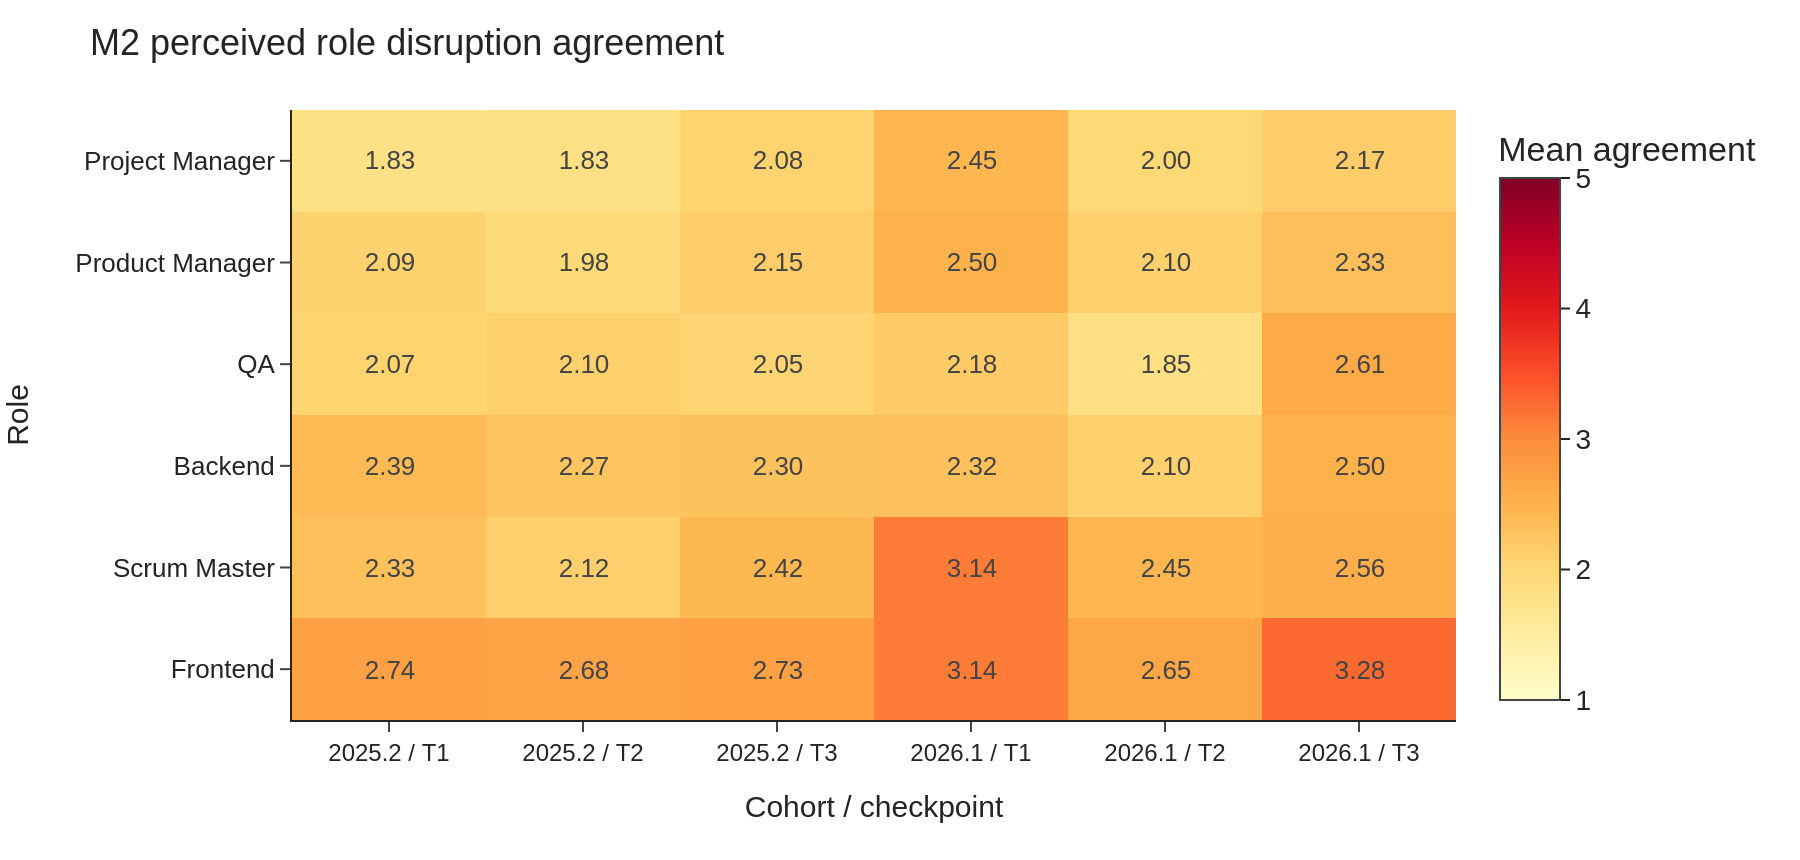
\includegraphics[width=\textwidth]{../figures/rq1_m2_role_perception_heatmap.png}
\caption{M2 perceived role-disruption agreement by cohort and checkpoint.
Cells show mean agreement on the $1$--$5$ Likert scale.}
\label{fig:rq1-m2}
\end{figure*}
% PROVENANCE: M2 distributions and role summaries are from
% paper_v9/data/metrics/m2_role_perception_distributions.csv and
% paper_v9/data/metrics/m2_role_perception_by_team_semester.csv. The metric
% metadata defines the scale as 1--5 Likert agreement and limits interpretation
% to perceived role disruption, not objective extinction risk.

The privacy-preserving paired sensitivity analysis reinforces this caution.
There are 38 paired respondents per role in 2025.2 and 16 per role in 2026.1.
Changes are mixed rather than uniformly directional: in 2025.2, Project
Manager shows the largest increase ($+0.32$) and Backend is nearly unchanged
($-0.03$); in 2026.1, QA increases by $+0.69$, while Scrum Master decreases
by $-0.31$. These paired values are sensitivity summaries, not causal or
population-level estimates.
% PROVENANCE: paired changes are from
% paper_v9/data/metrics/m2_role_perception_paired_t1_t3.csv and the executed
% paper_v9/verification_notebooks/verify_m2.ipynb. The paired analysis uses
% hashed anonymized respondent identifiers and is approved only as a
% privacy-preserving descriptive sensitivity analysis.

\subsection{RQ2: How does the temporal density of repository activity contrast with the qualitative typification of human coordination friction across the project lifecycle?}

RQ2 contrasts three descriptive evidence streams that operate at different
grains. M3 measures repository activity timing, author participation, and
concentration for 14 team-semesters. M4 measures clean source/test change at
team-semester and checkpoint grain. M5 counts candidate coordination markers
within a global transcript corpus by checkpoint. The measures are therefore
reported side by side as complementary descriptions, not as a common-scale
effect or a statistical correlation.
% PROVENANCE: RQ2 coverage and grains are declared in
% paper_v9/data/metrics/m3_author_activity_dynamics.metadata.json,
% m4_clean_change_dynamics.metadata.json, and
% m5_coordination_evidence.metadata.json.

M3 shows a pronounced concentration of repository activity around the final
evaluator anchor. In the semester-pooled rolling view, total commits increase
from $95$ at 21 days before the anchor to $159$ one day before, peak at $302$
one day after, and fall to $28$ at seven days after. At the anchor itself,
all 14 team-semesters have observed activity; at $-7$ days, only 5 of 14 are
active, and at $+7$ days, 7 of 14 remain active. The corresponding median
commit count per team-semester is $12.5$ at the anchor and $0.5$ at $+7$ days.
These rolling windows overlap, so adjacent points are temporal summaries rather
than independent observations.
Figure~\ref{fig:rq2-m3} visualizes this pooled temporal shape; the dashed line
marks the final evaluator anchor.

\begin{figure*}[t]
\centering
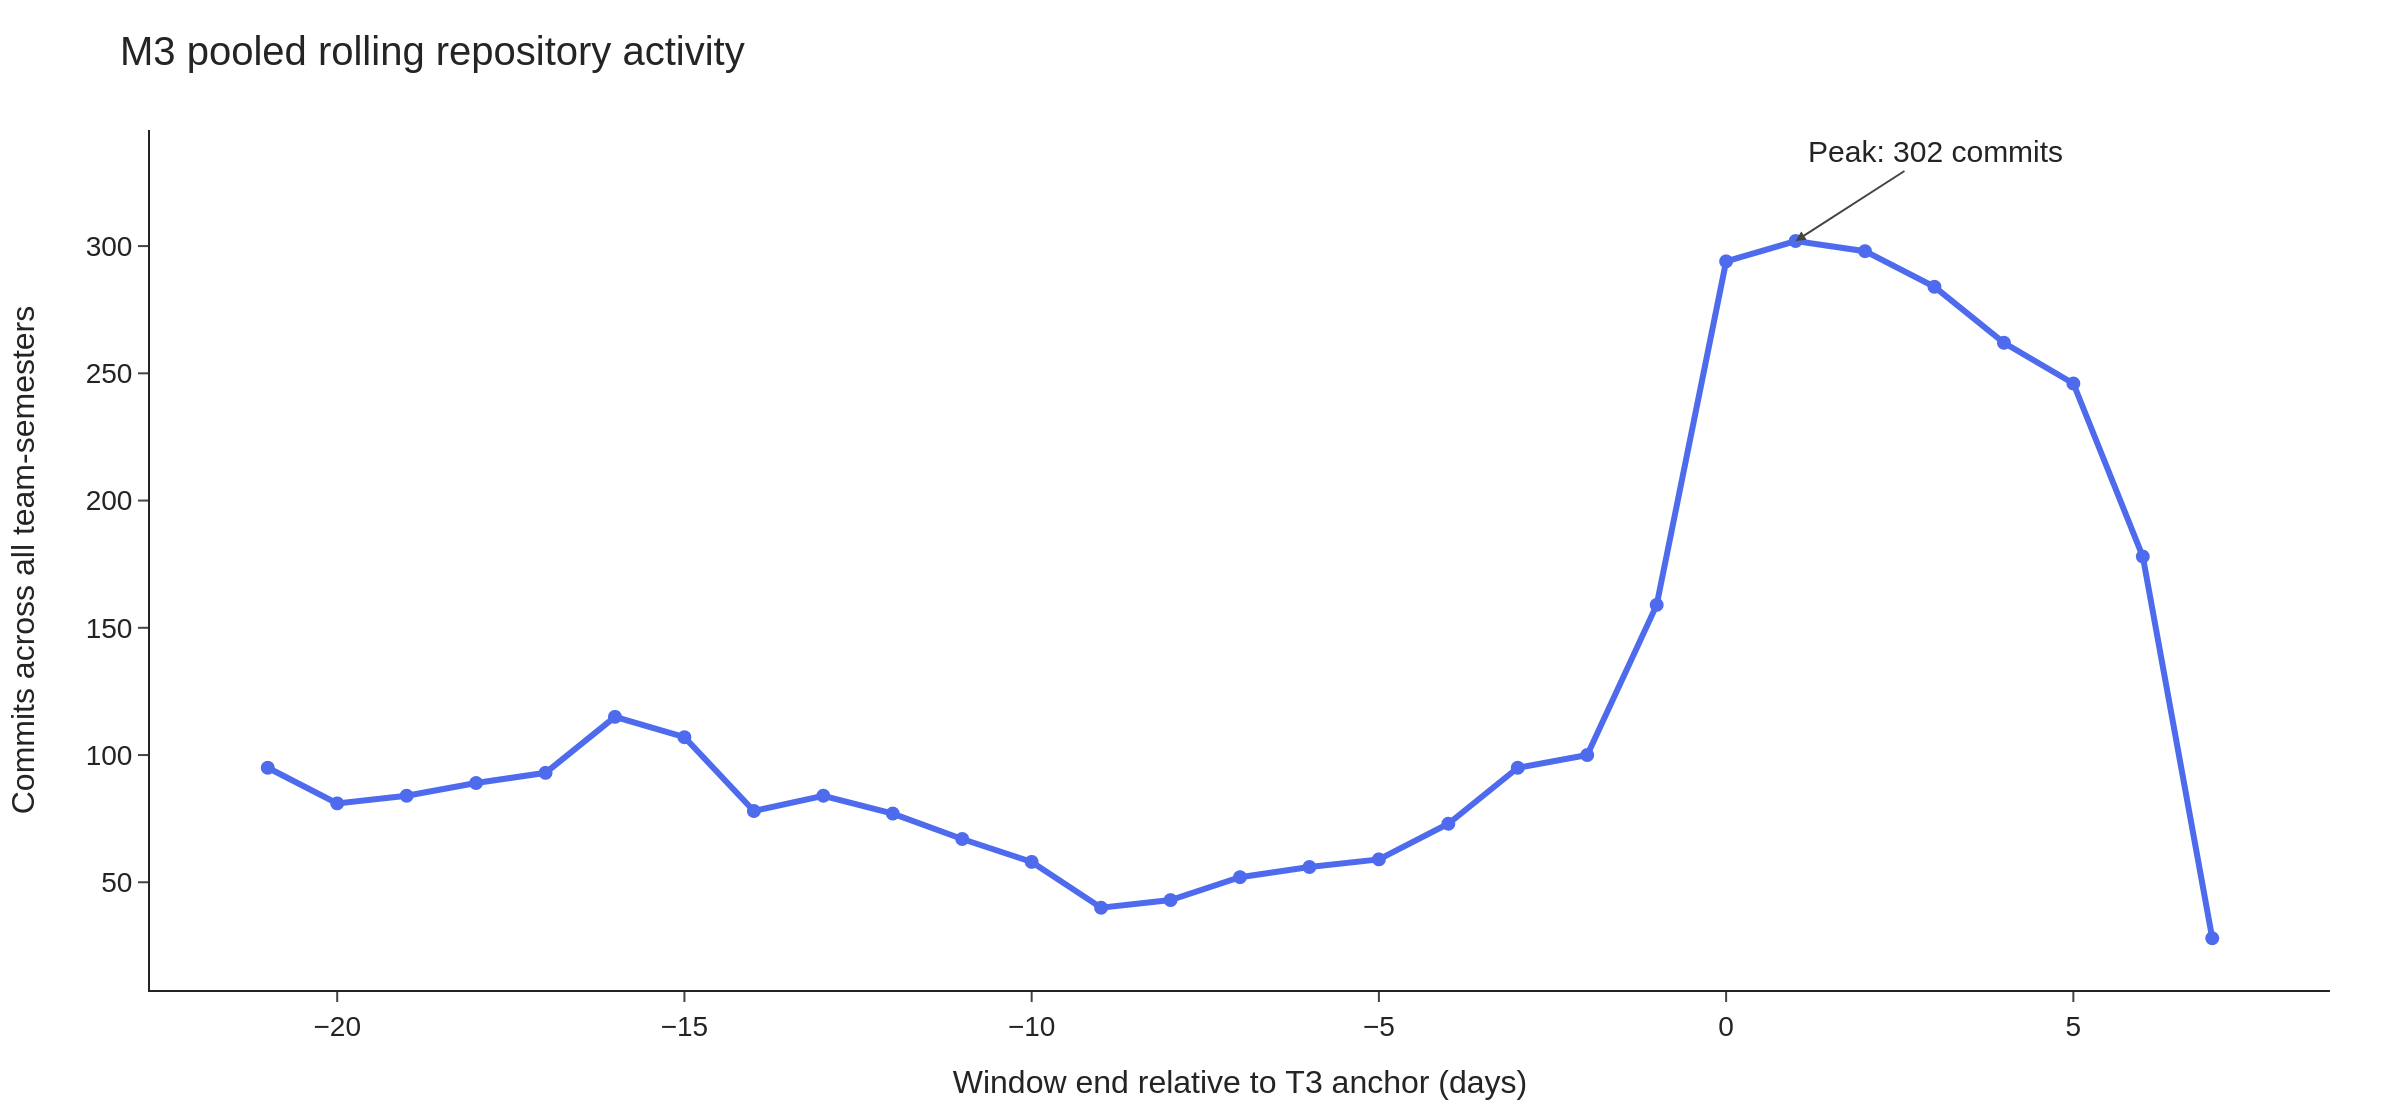
\includegraphics[width=\textwidth]{../figures/rq2_m3_activity_pooled.png}
\caption{M3 pooled rolling repository activity. The vertical marker identifies
the $T_3$ evaluator anchor; the annotation identifies the pooled peak.}
\label{fig:rq2-m3}
\end{figure*}
% PROVENANCE: Values are from
% paper_v9/data/metrics/m3_activity_rolling_7day_pooled.csv. The M3
% verification notebook is paper_v9/verification_notebooks/verify_m3.ipynb.

The checkpoint participation view shows the same concentration with substantial
heterogeneity. Across the 14 team-semesters, 7 have any post-checkpoint
activity. The final-window share of all commits ranges from $9.5\%$ to
$100.0\%$; three team-semesters have fewer than ten total commits, and their
shares should be treated as small-denominator descriptions. In the author
concentration output, the median pre-anchor window contains 12.5 commits,
3.5 active days, and 3 authors, with a median maximum-author share of $0.50$
and median Gini coefficient of $0.22$. Post-anchor windows are frequently
inactive; where activity exists, concentration statistics are not interpreted
for no-activity cases.
% PROVENANCE: Checkpoint and author summaries are from
% paper_v9/data/metrics/m3_author_activity_participation.csv and
% m3_author_concentration.csv. No author identity is exposed in these outputs.

M4 reproduces the temporal increase using a narrower clean-change definition.
Pooled clean churn rises from $21{,}718$ lines across 7 observed team-semesters
at $T_1$, to $47{,}545$ lines across 10 at $T_2$, and $136{,}325$ lines across
all 14 at $T_3$. The median clean churn per team-semester rises from $66.5$
lines at $T_1$ to $3{,}232.5$ at $T_2$ and $6{,}975.5$ at $T_3$. Clean change
accounts for $42.9\%$, $19.6\%$, and $1.0\%$ of all recorded churn at the
three checkpoints, respectively, because excluded or non-measurement paths
dominate the raw line-change total in the final checkpoint. This distinction is
why M4 is not interchangeable with total repository activity.
% PROVENANCE: M4 pooled endpoint values are from
% paper_v9/data/metrics/m4_churn_magnitude_pooled.csv and
% m4_artifact_composition_pooled.csv. The clean-path definition and its
% limitation are declared in m4_clean_change_dynamics.metadata.json.

M5 provides a separate textual axis for the 2025.2 transcript corpus. The
corpus contains 35, 37, and 28 transcript chunks at $T_1$, $T_2$, and $T_3$,
respectively, with two source sessions at each checkpoint. Candidate marker
density increases from $0.515$ to $1.132$ and $1.287$ markers per 1,000
transcript tokens. Marker counts are 12, 54, and 40, over 23,296, 47,705,
and 31,087 tokens. The composition also changes: integration markers account
for 20 of 54 markers at $T_2$, while blockers account for 7 of 40 at $T_3$.
These are deterministic lexical matches in a global corpus, not diagnoses of
coordination failure; transcript coverage is unavailable for 2026.1.
% PROVENANCE: M5 density, composition, coverage, lexicon, and audit rows are
% from paper_v9/data/metrics/m5_marker_density.csv,
% m5_marker_composition.csv, m5_corpus_coverage.csv,
% m5_lexicon.json, and m5_evidence_audit_trail.csv. No new LLM calls are
% required by M5.

Table~\ref{tab:rq2-summary} consolidates the principal RQ2 values while
retaining their distinct units and analytical grains. Figure~\ref{fig:rq2-m4-m5}
shows the M4 and M5 checkpoint trajectories in separate panels.

\begin{table*}[t]
\caption{RQ2 Temporal Summary with Explicit Units}
\label{tab:rq2-summary}
\centering
\scriptsize
\setlength{\tabcolsep}{5pt}
\begin{tabular}{@{}llccccc@{}}
\toprule
\textbf{Metric} & \textbf{Unit / grain} & \textbf{$T_1$ or $-7$} & \textbf{$T_2$ or $-1$} & \textbf{$T_3$ or $0$} & \textbf{Post-anchor} & \textbf{Coverage} \\
\midrule
M3 activity & Pooled commits / rolling window & 52 ($-7$) & 159 ($-1$) & 294 ($0$) & 302 ($+1$); 28 ($+7$) & 14 team-semesters \\
M4 clean change & Clean churn lines / checkpoint & 21,718 & 47,545 & 136,325 & -- & 7 / 10 / 14 observed \\
M5 lexical evidence & Markers per 1,000 tokens / global corpus & 0.515 & 1.132 & 1.287 & -- & 2025.2 only \\
\bottomrule
\end{tabular}
\end{table*}
% PROVENANCE: Table~\ref{tab:rq2-summary} is transcribed from
% paper_v9/data/metrics/m3_activity_rolling_7day_pooled.csv,
% m4_churn_magnitude_pooled.csv, and m5_marker_density.csv.

\begin{figure*}[t]
\centering
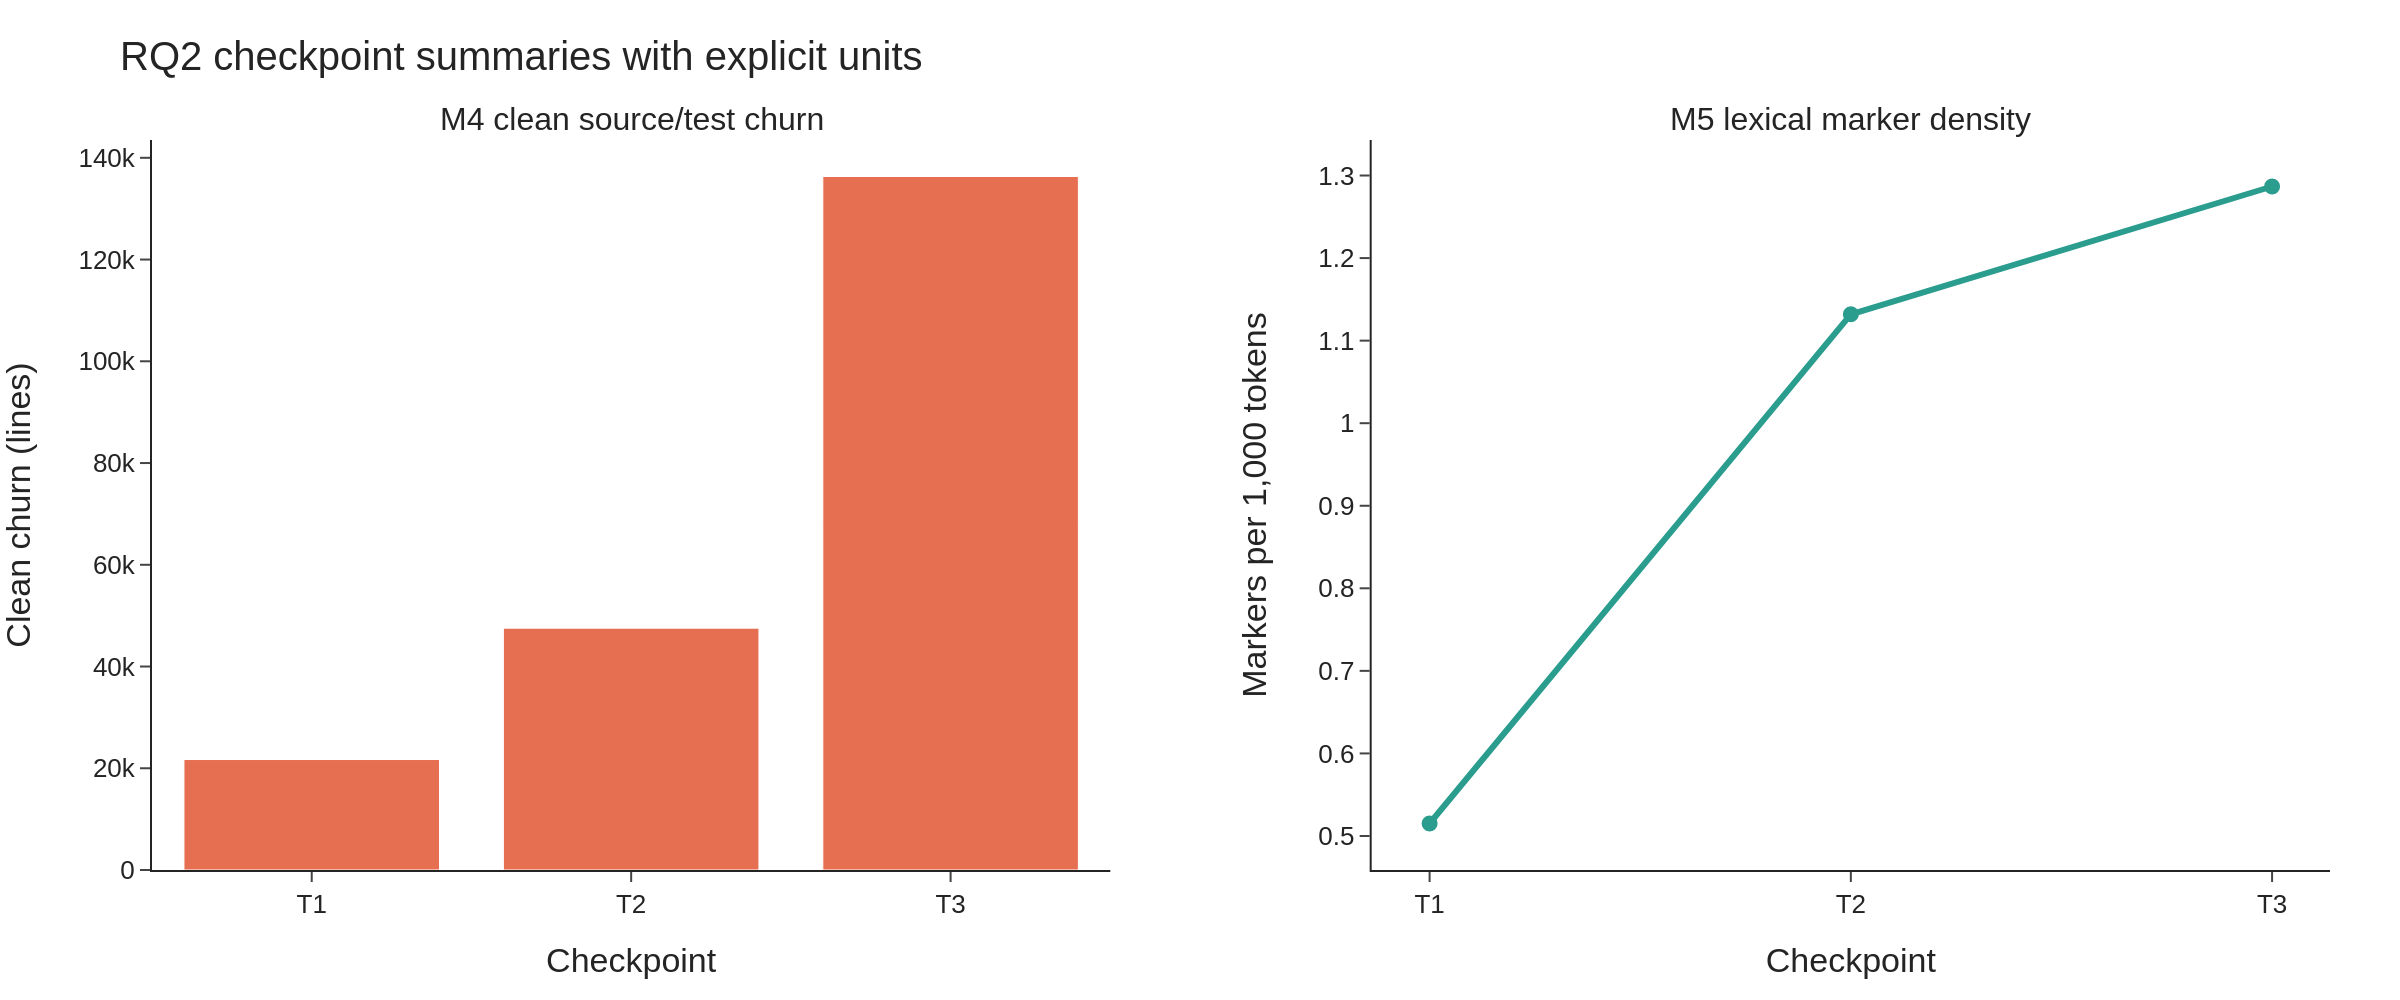
\includegraphics[width=\textwidth]{../figures/rq2_m4_m5_checkpoint_panels.png}
\caption{RQ2 checkpoint summaries with explicit units. M4 clean source/test
churn and M5 lexical marker density use separate panels and scales.}
\label{fig:rq2-m4-m5}
\end{figure*}

Taken together, M3 and M4 show that repository-visible activity and clean
source/test change become most concentrated near the final checkpoint, while
M5 shows an increase in candidate coordination-language density across the
observed 2025.2 transcript corpus. The three patterns are compatible with the
RQ2 descriptive contrast, but they do not establish that repository activity
causes coordination friction, that lexical markers measure friction without
error, or that the 2025.2 transcript trajectory generalizes to 2026.1.
